% Consolidated revision results for the FedHAD manuscript.
% Generated by analysis/revision_consolidated_tables_figures/consolidate.py -- regenerate rather than edit by hand.
%
% Preamble requirements:
%   \usepackage{booktabs}
%   \usepackage{graphicx}
%
% Paths assume this file is \input from the manuscript root with
% revision_consolidated_tables_figures/ copied in as-is. Adjust \graphicspath if not.

% ---------------------------------------------------------------- tables ----
% Generated by consolidate.py -- do not edit by hand.
% Requires \usepackage{booktabs}.
\begin{table*}[t]
\centering
\caption{Final accuracy and nominal training compute per method and dataset ($\alpha=0.5$ campaign, 30 seeds). Compute reduction is relative to FedAvg. Accuracy per TFLOP is reported as secondary information only; the primary efficiency evidence is Fig.~\ref{fig:pareto} and Table~\ref{tab:cost-to-target}.}
\label{tab:acc-compute}
\begin{tabular}{llrrrrr}
\toprule
Dataset & Method & $n$ & Final acc. (\%) & TFLOPs & Compute red. (\%) & Acc/TFLOP \\
\midrule
MNIST & FedAvg & 30 & 99.00 $\pm$ 0.11 & 4.56 & 0.0 & 0.217 \\
MNIST & FedAvgM & 30 & 98.34 $\pm$ 0.20 & 4.56 & 0.0 & 0.216 \\
MNIST & FedProx & 30 & 98.96 $\pm$ 0.09 & 4.56 & 0.0 & 0.217 \\
MNIST & FedNova & 30 & 98.98 $\pm$ 0.11 & 4.56 & 0.0 & 0.217 \\
MNIST & FedHAD & 30 & 98.91 $\pm$ 0.13 & 3.65 & 20.0 & 0.271 \\
\addlinespace
FashionMNIST & FedAvg & 30 & 88.34 $\pm$ 0.52 & 4.56 & 0.0 & 0.194 \\
FashionMNIST & FedAvgM & 30 & 85.23 $\pm$ 0.99 & 4.56 & 0.0 & 0.187 \\
FashionMNIST & FedProx & 30 & 88.35 $\pm$ 0.58 & 4.56 & 0.0 & 0.194 \\
FashionMNIST & FedNova & 30 & 88.38 $\pm$ 0.47 & 4.56 & 0.0 & 0.194 \\
FashionMNIST & FedHAD & 30 & 88.18 $\pm$ 0.54 & 3.65 & 20.1 & 0.242 \\
\addlinespace
CIFAR10 & FedAvg & 30 & 79.83 $\pm$ 1.39 & 407.03 & 0.0 & 0.002 \\
CIFAR10 & FedAvgM & 30 & 68.75 $\pm$ 2.52 & 407.03 & 0.0 & 0.002 \\
CIFAR10 & FedProx & 30 & 80.41 $\pm$ 1.21 & 407.03 & 0.0 & 0.002 \\
CIFAR10 & FedNova & 30 & 80.05 $\pm$ 1.12 & 407.03 & 0.0 & 0.002 \\
CIFAR10 & FedHAD & 30 & 80.21 $\pm$ 1.25 & 325.26 & 20.1 & 0.002 \\
\addlinespace
FEMNIST & FedAvg & 30 & 65.65 $\pm$ 1.07 & 12.39 & 0.0 & 0.053 \\
FEMNIST & FedAvgM & 30 & 64.93 $\pm$ 1.27 & 12.39 & 0.0 & 0.052 \\
FEMNIST & FedProx & 30 & 65.94 $\pm$ 1.36 & 12.39 & 0.0 & 0.053 \\
FEMNIST & FedNova & 30 & 65.00 $\pm$ 1.28 & 12.39 & 0.0 & 0.052 \\
FEMNIST & FedHAD & 30 & 65.11 $\pm$ 1.18 & 11.13 & 10.2 & 0.058 \\
\bottomrule
\end{tabular}

\vspace{2pt}
{\footnotesize\raggedright
\textit{Note.} FEMNIST includes the complete reruns of FedProx seed 66 and FedHAD seed 53. Fixed-epoch compute is the shared scheduled nominal workload; the raw reported value is retained in the audit CSV. The comparison uses a COMMON COMPUTE CEILING (baselines at 5 local epochs, FedHAD adaptive within 2--5), not a matched budget; matched-budget evidence is in Table~\ref{tab:ablation}.
\par}
\end{table*}

% Generated by consolidate.py -- do not edit by hand.
% Requires \usepackage{booktabs}.
\begin{table*}[t]
\centering
\caption{Final accuracy (\%) as heterogeneity increases. Values are means over the available seeds; standard deviations are in \texttt{data/blockB\_heterogeneity.csv}.}
\label{tab:heterogeneity}
\begin{tabular}{llrrrr}
\toprule
Dataset & Method & $\alpha=0.01$ & $\alpha=0.1$ & $\alpha=0.5$ & $\alpha=1$ \\
\midrule
MNIST & FedAvg & 93.06 & 97.66 & 99.00 & 99.09 \\
MNIST & FedAvgM & 89.03 & 95.31 & 98.34 & 98.35 \\
MNIST & FedProx & 88.77 & 96.86 & 98.96 & 99.08 \\
MNIST & FedNova & 91.82 & 98.03 & 98.98 & 99.09 \\
MNIST & FedHAD & 91.25 & 96.72 & 98.91 & 99.04 \\
\addlinespace
FashionMNIST & FedAvg & 69.39 & 82.15 & 88.34 & 88.98 \\
FashionMNIST & FedAvgM & 57.95 & 75.79 & 85.23 & 86.33 \\
FashionMNIST & FedProx & 66.18 & 80.60 & 88.35 & 89.18 \\
FashionMNIST & FedNova & 67.33 & 82.24 & 88.38 & 89.10 \\
FashionMNIST & FedHAD & 70.89 & 80.80 & 88.18 & 88.99 \\
\addlinespace
CIFAR10 & FedAvg & 54.25 & 68.91 & 79.83 & 81.71 \\
CIFAR10 & FedAvgM & 48.00 & 58.64 & 68.75 & 70.77 \\
CIFAR10 & FedProx & 53.33 & 67.62 & 80.41 & 81.85 \\
CIFAR10 & FedNova & 46.60 & 67.55 & 80.05 & 81.61 \\
CIFAR10 & FedHAD & 55.90 & 68.66 & 80.21 & 81.83 \\
\bottomrule
\end{tabular}

\vspace{2pt}
{\footnotesize\raggedright
\textit{Note.} Combines the $\alpha=0.5$ and $\alpha=0.01$ base campaigns, both run on the workstation declared in the manuscript. A dash means the combination was not executed; no value is imputed.
\par}
\end{table*}

% Generated by consolidate.py -- do not edit by hand.
% Requires \usepackage{booktabs}.
\begin{table*}[t]
\centering
\caption{Controlled ablation of FedHAD on CIFAR-10 (revision campaign, 30 seeds, fixed initialisation). Paired differences in final accuracy, with 95\% bootstrap intervals over seeds. Positive favours the first arm.}
\label{tab:ablation}
\begin{tabular}{llrrrlrr}
\toprule
\# & Contrast & $\alpha$ & $n$ & $\Delta$acc (pp) & 95\% CI & $d_z$ & $p$ \\
\midrule
Q1 & \texttt{full\_fedhad} $-$ \texttt{fixed\_matched} & 0.01 & 30 & +1.95$^{*}$ & [+1.23, +2.72] & +0.92 & $<0.001$ \\
Q1 & \texttt{full\_fedhad} $-$ \texttt{fixed\_matched} & 0.1 & 30 & +0.76$^{*}$ & [+0.16, +1.32] & +0.46 & 0.014 \\
Q2 & \texttt{full\_fedhad} $-$ \texttt{permuted\_allocation} & 0.01 & 30 & +0.80$^{*}$ & [+0.30, +1.30] & +0.56 & 0.006 \\
Q2 & \texttt{full\_fedhad} $-$ \texttt{permuted\_allocation} & 0.1 & 30 & +0.30 & [-0.23, +0.83] & +0.20 & 0.328 \\
Q3 & \texttt{epoch\_only} $-$ \texttt{fixed\_matched} & 0.01 & 30 & +1.01$^{*}$ & [+0.22, +1.83] & +0.44 & 0.038 \\
Q3 & \texttt{epoch\_only} $-$ \texttt{fixed\_matched} & 0.1 & 30 & -0.42 & [-1.08, +0.17] & -0.24 & 0.229 \\
Q4 & \texttt{lr\_only\_matched} $-$ \texttt{fixed\_matched} & 0.01 & 30 & +1.81$^{*}$ & [+1.09, +2.58] & +0.84 & $<0.001$ \\
Q4 & \texttt{lr\_only\_matched} $-$ \texttt{fixed\_matched} & 0.1 & 30 & +0.71$^{*}$ & [+0.25, +1.21] & +0.52 & 0.010 \\
Q5a & \texttt{full\_fedhad} $-$ \texttt{epoch\_only} & 0.01 & 30 & +0.94 & [+0.13, +1.84] & +0.38 & 0.096 \\
Q5a & \texttt{full\_fedhad} $-$ \texttt{epoch\_only} & 0.1 & 30 & +1.18$^{*}$ & [+0.64, +1.71] & +0.78 & $<0.001$ \\
Q5b & \texttt{full\_fedhad} $-$ \texttt{lr\_only\_matched} & 0.01 & 30 & +0.14 & [-0.64, +0.93] & +0.06 & 0.926 \\
Q5b & \texttt{full\_fedhad} $-$ \texttt{lr\_only\_matched} & 0.1 & 30 & +0.04 & [-0.49, +0.55] & +0.03 & 0.655 \\
\bottomrule
\end{tabular}

\vspace{2pt}
{\footnotesize\raggedright
\textit{Note.} Every arm of a cell shares initial weights, partitions, clients and $H_k$ (SHA-256 verified). Compute is measured as minibatch updates. \texttt{epoch\_only} matches \texttt{full\_fedhad} exactly, and \texttt{lr\_only\_matched} matches \texttt{fixed\_matched} exactly. The fixed allocation is budget-matched relative to \texttt{full\_fedhad} within a median 0.26\% (max 3.44\%); thus Q1, Q3 and Q5b are approximate budget-matched contrasts, whereas Q4 and Q5a are exact in updates. \texttt{permuted\_allocation} is \textbf{not} an equal-compute arm -- its update total deviates by a median -1.53\% (range -15.51 to +13.11\%) because epochs are integers, there are five clients and each holds a different number of minibatches; it is reported as complementary evidence on the client-to-budget association only. $^{*}$ marks $p<0.05$; a non-significant row is a failure to detect a difference at this sample size, never evidence of equivalence.
\par}
\end{table*}

% Generated by consolidate.py -- do not edit by hand.
% Requires \usepackage{booktabs}.
\begin{table*}[t]
\centering
\caption{Long-horizon runs (50 communication rounds, CIFAR-10).}
\label{tab:long-horizon}
\begin{tabular}{lllrrrrr}
\toprule
Campaign & $\alpha$ & Method & $n$ & Final acc. (\%) & Best acc. (\%) & TFLOPs & Wall-clock (s) \\
\midrule
base\_alpha\_0.01 & 0.01 & FedAvg & 30 & 64.40 $\pm$ 3.39 & 65.42 & 2035.15 & 784 \\
base\_alpha\_0.01 & 0.01 & FedAvgM & 30 & 56.73 $\pm$ 4.40 & 58.85 & 2035.15 & 783 \\
base\_alpha\_0.01 & 0.01 & FedHAD & 30 & 65.81 $\pm$ 2.68 & 66.19 & 1313.94 & 845 \\
base\_alpha\_0.01 & 0.01 & FedProx & 30 & 64.97 $\pm$ 2.97 & 65.44 & 2035.15 & 1093 \\
base\_alpha\_0.5 & 0.5 & FedAvg & 30 & 80.60 $\pm$ 0.89 & 81.02 & 2035.16 & 1913 \\
base\_alpha\_0.5 & 0.5 & FedAvgM & 30 & 78.04 $\pm$ 1.04 & 78.59 & 2035.16 & 1905 \\
base\_alpha\_0.5 & 0.5 & FedHAD & 30 & 81.80 $\pm$ 0.64 & 82.17 & 1626.28 & 2254 \\
base\_alpha\_0.5 & 0.5 & FedProx & 30 & 81.77 $\pm$ 0.89 & 82.09 & 2035.16 & 2774 \\
\bottomrule
\end{tabular}

\vspace{2pt}
{\footnotesize\raggedright
\textit{Note.} The two campaigns are reported side by side and never pooled: they differ in $\alpha$ and were executed separately. Wall-clock is reported as recorded; the machine was not otherwise controlled.
\par}
\end{table*}

% Generated by consolidate.py -- do not edit by hand.
% Requires \usepackage{booktabs}.
\begin{table*}[t]
\centering
\caption{FedNova in the scenarios where it was executed, shown alongside the other methods in exactly those scenarios.}
\label{tab:fednova}
\begin{tabular}{lllrrrr}
\toprule
Experiment & Dataset & $\alpha$ & Method & $n$ & Final acc. (\%) & TFLOPs \\
\midrule
test1\_convergencia & CIFAR10 & 0.5 & FedAvg & 30 & 79.83 $\pm$ 1.39 & 407.03 \\
test1\_convergencia & CIFAR10 & 0.5 & FedAvgM & 30 & 68.75 $\pm$ 2.52 & 407.03 \\
test1\_convergencia & CIFAR10 & 0.5 & FedProx & 30 & 80.41 $\pm$ 1.21 & 407.03 \\
test1\_convergencia & CIFAR10 & 0.5 & FedNova & 30 & 80.05 $\pm$ 1.12 & 407.03 \\
test1\_convergencia & CIFAR10 & 0.5 & FedHAD & 30 & 80.21 $\pm$ 1.25 & 325.26 \\
\addlinespace
test1\_convergencia & FashionMNIST & 0.5 & FedAvg & 30 & 88.34 $\pm$ 0.52 & 4.56 \\
test1\_convergencia & FashionMNIST & 0.5 & FedAvgM & 30 & 85.23 $\pm$ 0.99 & 4.56 \\
test1\_convergencia & FashionMNIST & 0.5 & FedProx & 30 & 88.35 $\pm$ 0.58 & 4.56 \\
test1\_convergencia & FashionMNIST & 0.5 & FedNova & 30 & 88.38 $\pm$ 0.47 & 4.56 \\
test1\_convergencia & FashionMNIST & 0.5 & FedHAD & 30 & 88.18 $\pm$ 0.54 & 3.65 \\
\addlinespace
test1\_convergencia & MNIST & 0.5 & FedAvg & 30 & 99.00 $\pm$ 0.11 & 4.56 \\
test1\_convergencia & MNIST & 0.5 & FedAvgM & 30 & 98.34 $\pm$ 0.20 & 4.56 \\
test1\_convergencia & MNIST & 0.5 & FedProx & 30 & 98.96 $\pm$ 0.09 & 4.56 \\
test1\_convergencia & MNIST & 0.5 & FedNova & 30 & 98.98 $\pm$ 0.11 & 4.56 \\
test1\_convergencia & MNIST & 0.5 & FedHAD & 30 & 98.91 $\pm$ 0.13 & 3.65 \\
\addlinespace
test2\_robustez\_alpha & CIFAR10 & 0.01 & FedAvg & 30 & 54.16 $\pm$ 5.46 & 407.03 \\
test2\_robustez\_alpha & CIFAR10 & 0.01 & FedAvgM & 30 & 46.84 $\pm$ 4.35 & 407.03 \\
test2\_robustez\_alpha & CIFAR10 & 0.01 & FedProx & 30 & 52.94 $\pm$ 4.65 & 407.03 \\
test2\_robustez\_alpha & CIFAR10 & 0.01 & FedNova & 30 & 46.60 $\pm$ 7.12 & 407.03 \\
test2\_robustez\_alpha & CIFAR10 & 0.01 & FedHAD & 30 & 55.78 $\pm$ 4.05 & 262.79 \\
\addlinespace
test2\_robustez\_alpha & CIFAR10 & 0.1 & FedAvg & 30 & 69.03 $\pm$ 2.93 & 407.03 \\
test2\_robustez\_alpha & CIFAR10 & 0.1 & FedAvgM & 30 & 58.44 $\pm$ 3.53 & 407.03 \\
test2\_robustez\_alpha & CIFAR10 & 0.1 & FedProx & 30 & 67.85 $\pm$ 3.00 & 407.03 \\
test2\_robustez\_alpha & CIFAR10 & 0.1 & FedNova & 30 & 67.55 $\pm$ 3.63 & 407.03 \\
test2\_robustez\_alpha & CIFAR10 & 0.1 & FedHAD & 30 & 68.53 $\pm$ 3.22 & 288.71 \\
\addlinespace
test2\_robustez\_alpha & CIFAR10 & 1 & FedAvg & 30 & 81.69 $\pm$ 0.49 & 407.03 \\
test2\_robustez\_alpha & CIFAR10 & 1 & FedAvgM & 30 & 70.73 $\pm$ 2.55 & 407.03 \\
test2\_robustez\_alpha & CIFAR10 & 1 & FedProx & 30 & 82.01 $\pm$ 0.45 & 407.03 \\
test2\_robustez\_alpha & CIFAR10 & 1 & FedNova & 30 & 81.61 $\pm$ 0.55 & 407.03 \\
test2\_robustez\_alpha & CIFAR10 & 1 & FedHAD & 30 & 82.04 $\pm$ 0.50 & 330.01 \\
\addlinespace
test2\_robustez\_alpha & FashionMNIST & 0.01 & FedAvg & 30 & 69.95 $\pm$ 7.15 & 4.56 \\
test2\_robustez\_alpha & FashionMNIST & 0.01 & FedAvgM & 30 & 58.17 $\pm$ 12.20 & 4.56 \\
test2\_robustez\_alpha & FashionMNIST & 0.01 & FedProx & 30 & 66.53 $\pm$ 5.10 & 4.56 \\
test2\_robustez\_alpha & FashionMNIST & 0.01 & FedNova & 30 & 67.33 $\pm$ 9.38 & 4.56 \\
test2\_robustez\_alpha & FashionMNIST & 0.01 & FedHAD & 30 & 70.72 $\pm$ 3.14 & 2.95 \\
\addlinespace
test2\_robustez\_alpha & FashionMNIST & 0.1 & FedAvg & 30 & 81.85 $\pm$ 3.37 & 4.56 \\
test2\_robustez\_alpha & FashionMNIST & 0.1 & FedAvgM & 30 & 73.97 $\pm$ 5.16 & 4.56 \\
test2\_robustez\_alpha & FashionMNIST & 0.1 & FedProx & 30 & 80.80 $\pm$ 3.41 & 4.56 \\
test2\_robustez\_alpha & FashionMNIST & 0.1 & FedNova & 30 & 82.24 $\pm$ 2.56 & 4.56 \\
test2\_robustez\_alpha & FashionMNIST & 0.1 & FedHAD & 30 & 81.01 $\pm$ 2.92 & 3.24 \\
\addlinespace
test2\_robustez\_alpha & FashionMNIST & 1 & FedAvg & 30 & 88.96 $\pm$ 0.32 & 4.56 \\
test2\_robustez\_alpha & FashionMNIST & 1 & FedAvgM & 30 & 85.99 $\pm$ 0.86 & 4.56 \\
test2\_robustez\_alpha & FashionMNIST & 1 & FedProx & 30 & 88.99 $\pm$ 0.33 & 4.56 \\
test2\_robustez\_alpha & FashionMNIST & 1 & FedNova & 30 & 89.10 $\pm$ 0.24 & 4.56 \\
test2\_robustez\_alpha & FashionMNIST & 1 & FedHAD & 30 & 89.09 $\pm$ 0.33 & 3.70 \\
\addlinespace
test2\_robustez\_alpha & MNIST & 0.01 & FedAvg & 30 & 93.24 $\pm$ 2.76 & 4.56 \\
test2\_robustez\_alpha & MNIST & 0.01 & FedAvgM & 30 & 90.18 $\pm$ 2.89 & 4.56 \\
test2\_robustez\_alpha & MNIST & 0.01 & FedProx & 30 & 88.67 $\pm$ 3.36 & 4.56 \\
test2\_robustez\_alpha & MNIST & 0.01 & FedNova & 30 & 91.82 $\pm$ 4.58 & 4.56 \\
test2\_robustez\_alpha & MNIST & 0.01 & FedHAD & 30 & 91.14 $\pm$ 2.61 & 2.94 \\
\addlinespace
test2\_robustez\_alpha & MNIST & 0.1 & FedAvg & 30 & 97.67 $\pm$ 0.59 & 4.56 \\
test2\_robustez\_alpha & MNIST & 0.1 & FedAvgM & 30 & 95.19 $\pm$ 2.09 & 4.56 \\
test2\_robustez\_alpha & MNIST & 0.1 & FedProx & 30 & 96.72 $\pm$ 1.40 & 4.56 \\
test2\_robustez\_alpha & MNIST & 0.1 & FedNova & 30 & 98.03 $\pm$ 0.44 & 4.56 \\
test2\_robustez\_alpha & MNIST & 0.1 & FedHAD & 30 & 96.76 $\pm$ 1.22 & 3.23 \\
\addlinespace
test2\_robustez\_alpha & MNIST & 1 & FedAvg & 30 & 99.11 $\pm$ 0.07 & 4.56 \\
test2\_robustez\_alpha & MNIST & 1 & FedAvgM & 30 & 98.27 $\pm$ 0.73 & 4.56 \\
test2\_robustez\_alpha & MNIST & 1 & FedProx & 30 & 99.05 $\pm$ 0.09 & 4.56 \\
test2\_robustez\_alpha & MNIST & 1 & FedNova & 30 & 99.09 $\pm$ 0.07 & 4.56 \\
test2\_robustez\_alpha & MNIST & 1 & FedHAD & 30 & 99.06 $\pm$ 0.10 & 3.70 \\
\bottomrule
\end{tabular}

\vspace{2pt}
{\footnotesize\raggedright
\textit{Note.} FedNova was run only for convergence (CD1), robustness (CD2) and FEMNIST (CD8) in the $\alpha=0.5$ campaign. Absent combinations are omitted rather than imputed.
\par}
\end{table*}

% Generated by consolidate.py -- do not edit by hand.
% Requires \usepackage{booktabs}.
\begin{table}[t]
\centering
\caption{Validation of $H_k$ as a drift proxy: Spearman correlation between $H_k$ and the per-client update diagnostics.}
\label{tab:proxy}
\begin{tabular}{lrrrr}
\toprule
Method & $\alpha$ & $n$ & $\rho(H_k,\cos)$ & $\rho(H_k,\|\Delta\|/\text{step})$ \\
\midrule
FedAvg & 0.01 & 470 & -0.962 & +0.408 \\
FedAvg & 0.1 & 500 & -0.908 & +0.656 \\
FedAvg & 1 & 500 & -0.445 & +0.320 \\
FedAvgM & 0.01 & 470 & -0.968 & +0.696 \\
FedAvgM & 0.1 & 500 & -0.923 & +0.748 \\
FedAvgM & 1 & 500 & -0.469 & +0.327 \\
FedProx & 0.01 & 470 & -0.971 & +0.321 \\
FedProx & 0.1 & 500 & -0.911 & +0.728 \\
FedProx & 1 & 500 & -0.455 & +0.375 \\
FedHAD & 0.01 & 470 & -0.970 & +0.832 \\
FedHAD & 0.1 & 500 & -0.928 & +0.803 \\
FedHAD & 1 & 500 & -0.527 & +0.263 \\
\bottomrule
\end{tabular}

\vspace{2pt}
{\footnotesize\raggedright
\textit{Note.} Three (alpha, seed, client) pairs with $n_k=0$ are excluded: their logged values are sentinels, not measurements. In FedHAD $H_k$ also drives $E_k$ and the learning rate, so its correlation is not an independent validation; the three baselines, where $H_k$ is purely observational, are the clean estimates.
\par}
\end{table}

% Generated from global_prior_analysis/tables/T3--T6 by generate_femnist_global_prior_table.py.
% Requires \usepackage{booktabs}.
\begin{table}[t]
\centering
\caption{Empirical global class prior and its operational implications on FEMNIST. The prior is aggregated over 2{,}095 distinct writers and compared with the uniform reference implicitly assumed by the normalised coefficient of variation used as $H_k$.}
\label{tab:femnist-global-prior}
\begin{tabular}{lr}
\toprule
Quantity & Value \\
\midrule
\multicolumn{2}{l}{\emph{Global class prior}} \\
Classes / examples & 62 / 472{,}734 \\
Uniform probability per class & 1.613\% \\
Empirical class probability, min--max & 0.271--5.511\% \\
Most/least frequent-class ratio & 20.4$\times$ \\
Maximum deviation from uniform & 3.898 pp \\
JS(global $\parallel$ uniform), bits & 0.156 \\
\addlinespace
\multicolumn{2}{l}{\emph{Metric disagreement over writers}} \\
Spearman $\rho$, CV vs. JS ranking & 0.691 \\
Writers changing heterogeneity tercile & 756 / 2095 (36.1\%) \\
Writers changing local-epoch allocation & 504 / 2095 (24.1\%) \\
Total epoch budget, CV / remapped JS & 9226 / 9226 \\
\bottomrule
\end{tabular}
\vspace{2pt}
{\footnotesize\raggedright \textit{Note.} JS denotes Jensen--Shannon divergence from the empirical global prior. The JS scores were quantile matched to the CV scores, preserving the aggregate epoch budget; this is an offline counterfactual remapping rather than a trained FedHAD variant. FEMNIST has no client-drift telemetry, so these results establish a scope boundary for the uniform-prior assumption but do not compare the metrics' ability to predict drift or improve accuracy.\par}
\end{table}

% Generated by consolidate.py -- do not edit by hand.
% Requires \usepackage{booktabs}.
\begin{table}[t]
\centering
\caption{Association between four heterogeneity statistics and the raw client-update alignment measure on CIFAR-10 (Spearman $\rho$ against the cosine with the self-inclusive aggregate; baselines only).}
\label{tab:prior-metrics}
\begin{tabular}{lrrrrr}
\toprule
Method & $\alpha$ & Normalised CV & $1-$entropy & JS vs global & TV vs global \\
\midrule
FedAvg & 0.01 & -0.961 & -0.963 & -0.958 & -0.939 \\
FedAvg & 0.1 & -0.908 & -0.868 & -0.793 & -0.783 \\
FedAvg & 1 & -0.445 & -0.447 & -0.418 & -0.394 \\
FedAvgM & 0.01 & -0.967 & -0.968 & -0.964 & -0.943 \\
FedAvgM & 0.1 & -0.923 & -0.883 & -0.807 & -0.795 \\
FedAvgM & 1 & -0.469 & -0.469 & -0.438 & -0.416 \\
FedProx & 0.01 & -0.970 & -0.972 & -0.968 & -0.952 \\
FedProx & 0.1 & -0.911 & -0.872 & -0.799 & -0.790 \\
FedProx & 1 & -0.455 & -0.456 & -0.428 & -0.406 \\
\bottomrule
\end{tabular}

\vspace{2pt}
{\footnotesize\raggedright
\textit{Note.} CIFAR-10's empirical global prior is exactly uniform (5{,}000 images per class), so JS against the empirical and against the uniform prior coincide and this dataset cannot test the uniform-prior premise -- it characterises the regime where the premise holds. FEMNIST, whose pooled global prior is 20.4$\times$ skewed, lies outside that regime; see \texttt{data/blockG\_femnist\_prior.csv}.
\par}
\end{table}

% Generated by consolidate.py -- do not edit by hand.
% Requires \usepackage{booktabs}.
\begin{table*}[t]
\centering
\caption{Verification that every method operates on identical client partitions.}
\label{tab:partitions}
\begin{tabular}{llrrrrrr}
\toprule
Dataset & Partitioning & Scenarios & Methods & Identical indices & Identical counts & Negative control & RNG stress \\
\midrule
CIFAR10 & dirichlet & 360 & 5 & 360/360 & 360/360 & 360/360 & 360/360 \\
FEMNIST & natural & 30 & 5 & 30/30 & 30/30 & 30/30 & 30/30 \\
FashionMNIST & dirichlet & 360 & 5 & 360/360 & 360/360 & 360/360 & 360/360 \\
MNIST & dirichlet & 360 & 5 & 360/360 & 360/360 & 360/360 & 360/360 \\
\bottomrule
\end{tabular}

\vspace{2pt}
{\footnotesize\raggedright
\textit{Note.} Identity holds by construction: \texttt{dirichlet\_split\_noniid} reseeds NumPy as its first statement, making the partition a pure function of (labels, clients, $\alpha$, seed). The negative control confirms distinct seeds give distinct partitions; the RNG stress test consumes ${\sim}1.5$M draws and reseeds to 999 immediately before partitioning.
\par}
\end{table*}

\begin{table*}[t]
\centering
\caption{FedHAD and baselines across datasets and heterogeneity regimes. Each cell reports final accuracy in percent (top: mean $\pm$ standard deviation over 30 paired seeds) and mean training TFLOPs (bottom). FedHAD is bolded. All methods use identical client partitions for each seed.}
\label{tab:fedhad_all_baselines_compact}
\scriptsize
\setlength{\tabcolsep}{3.2pt}
\begin{tabular}{llccccc}
\toprule
\textbf{Dataset} & \textbf{Setting} & \textbf{FedHAD} & \textbf{FedAvg} & \textbf{FedAvgM} & \textbf{FedProx} & \textbf{FedNova} \\
\midrule
MNIST & $\alpha = 1.0$ & \textbf{\shortstack{99.06 $\pm$ 0.10 \\3.70}} & \shortstack{99.11 $\pm$ 0.07 \\4.56} & \shortstack{98.27 $\pm$ 0.73 \\4.56} & \shortstack{99.05 $\pm$ 0.09 \\4.56} & \shortstack{99.09 $\pm$ 0.07 \\4.56} \\
MNIST & $\alpha = 0.1$ & \textbf{\shortstack{96.76 $\pm$ 1.22 \\3.23}} & \shortstack{97.67 $\pm$ 0.59 \\4.56} & \shortstack{95.19 $\pm$ 2.09 \\4.56} & \shortstack{96.72 $\pm$ 1.40 \\4.56} & \shortstack{98.03 $\pm$ 0.44 \\4.56} \\
MNIST & $\alpha = 0.01$ & \textbf{\shortstack{91.14 $\pm$ 2.61 \\2.94}} & \shortstack{93.24 $\pm$ 2.76 \\4.56} & \shortstack{90.18 $\pm$ 2.89 \\4.56} & \shortstack{88.67 $\pm$ 3.36 \\4.56} & \shortstack{91.82 $\pm$ 4.58 \\4.56} \\
\midrule
FashionMNIST & $\alpha = 1.0$ & \textbf{\shortstack{89.09 $\pm$ 0.33 \\3.70}} & \shortstack{88.96 $\pm$ 0.32 \\4.56} & \shortstack{85.99 $\pm$ 0.86 \\4.56} & \shortstack{88.99 $\pm$ 0.33 \\4.56} & \shortstack{89.10 $\pm$ 0.24 \\4.56} \\
FashionMNIST & $\alpha = 0.1$ & \textbf{\shortstack{81.01 $\pm$ 2.92 \\3.24}} & \shortstack{81.85 $\pm$ 3.37 \\4.56} & \shortstack{73.97 $\pm$ 5.16 \\4.56} & \shortstack{80.80 $\pm$ 3.41 \\4.56} & \shortstack{82.24 $\pm$ 2.56 \\4.56} \\
FashionMNIST & $\alpha = 0.01$ & \textbf{\shortstack{70.72 $\pm$ 3.14 \\2.95}} & \shortstack{69.95 $\pm$ 7.15 \\4.56} & \shortstack{58.17 $\pm$ 12.20 \\4.56} & \shortstack{66.53 $\pm$ 5.10 \\4.56} & \shortstack{67.33 $\pm$ 9.38 \\4.56} \\
\midrule
CIFAR-10 & $\alpha = 1.0$ & \textbf{\shortstack{82.04 $\pm$ 0.50 \\330.01}} & \shortstack{81.69 $\pm$ 0.49 \\407.03} & \shortstack{70.73 $\pm$ 2.55 \\407.03} & \shortstack{82.01 $\pm$ 0.45 \\407.03} & \shortstack{81.61 $\pm$ 0.55 \\407.03} \\
CIFAR-10 & $\alpha = 0.1$ & \textbf{\shortstack{68.53 $\pm$ 3.22 \\288.71}} & \shortstack{69.03 $\pm$ 2.93 \\407.03} & \shortstack{58.44 $\pm$ 3.53 \\407.03} & \shortstack{67.85 $\pm$ 3.00 \\407.03} & \shortstack{67.55 $\pm$ 3.63 \\407.03} \\
CIFAR-10 & $\alpha = 0.01$ & \textbf{\shortstack{55.78 $\pm$ 4.05 \\262.79}} & \shortstack{54.16 $\pm$ 5.46 \\407.03} & \shortstack{46.84 $\pm$ 4.35 \\407.03} & \shortstack{52.94 $\pm$ 4.65 \\407.03} & \shortstack{46.60 $\pm$ 7.12 \\407.03} \\
\midrule
FEMNIST & natural & \textbf{\shortstack{65.11 $\pm$ 1.18 \\11.13}} & \shortstack{65.65 $\pm$ 1.07 \\12.39} & \shortstack{64.93 $\pm$ 1.27 \\12.39} & \shortstack{65.94 $\pm$ 1.36 \\12.39} & \shortstack{65.00 $\pm$ 1.28 \\12.39} \\
\bottomrule
\end{tabular}
\end{table*}

\begin{table*}[t]
\centering
\caption{Paired FedHAD versus FedNova comparison across datasets and heterogeneity regimes. Accuracy is mean $\pm$ standard deviation over 30 paired seeds. $\Delta$Acc is FedHAD minus FedNova in percentage points; brackets give the 95\% bootstrap interval of the paired mean. $p_{\mathrm{W}}$ is the two-sided Wilcoxon signed-rank $p$-value. Positive $\Delta$FLOPs denotes training-FLOP savings by FedHAD.}
\label{tab:fednova_comparison}
\scriptsize
\setlength{\tabcolsep}{3.2pt}
\begin{tabular}{llcccccc}
\toprule
\textbf{Dataset} &
\textbf{Setting} &
\textbf{FedHAD acc.} &
\textbf{FedNova acc.} &
\textbf{$\Delta$Acc (pp) [95\% CI]} &
\textbf{$p_{\mathrm{W}}$} &
\textbf{TFLOPs (HAD / Nova)} &
\textbf{$\Delta$FLOPs} \\
\midrule
MNIST & $\alpha = 1.0$ & 99.06 $\pm$ 0.10 & 99.09 $\pm$ 0.07 & -0.03 [-0.07, +0.00] & 0.081 & 3.70 / 4.56 & +18.9\% \\
MNIST & $\alpha = 0.1$ & 96.76 $\pm$ 1.22 & 98.03 $\pm$ 0.44 & -1.27 [-1.62, -0.94] & $<0.001$ & 3.23 / 4.56 & +29.2\% \\
MNIST & $\alpha = 0.01$ & 91.14 $\pm$ 2.61 & 91.82 $\pm$ 4.58 & -0.69 [-2.06, +0.86] & 0.146 & 2.94 / 4.56 & +35.5\% \\
FashionMNIST & $\alpha = 1.0$ & 89.09 $\pm$ 0.33 & 89.10 $\pm$ 0.24 & -0.01 [-0.15, +0.12] & 0.984 & 3.70 / 4.56 & +18.9\% \\
FashionMNIST & $\alpha = 0.1$ & 81.01 $\pm$ 2.92 & 82.24 $\pm$ 2.56 & -1.23 [-2.19, -0.30] & 0.023 & 3.24 / 4.56 & +29.1\% \\
FashionMNIST & $\alpha = 0.01$ & 70.72 $\pm$ 3.14 & 67.33 $\pm$ 9.38 & +3.38 [+0.10, +6.87] & 0.146 & 2.95 / 4.56 & +35.4\% \\
CIFAR-10 & $\alpha = 1.0$ & 82.04 $\pm$ 0.50 & 81.61 $\pm$ 0.55 & +0.43 [+0.26, +0.61] & $<0.001$ & 330.01 / 407.03 & +18.9\% \\
CIFAR-10 & $\alpha = 0.1$ & 68.53 $\pm$ 3.22 & 67.55 $\pm$ 3.63 & +0.98 [-0.25, +2.22] & 0.233 & 288.71 / 407.03 & +29.1\% \\
CIFAR-10 & $\alpha = 0.01$ & 55.78 $\pm$ 4.05 & 46.60 $\pm$ 7.12 & +9.17 [+6.29, +12.14] & $<0.001$ & 262.79 / 407.03 & +35.4\% \\
FEMNIST & natural federation & 65.11 $\pm$ 1.18 & 65.00 $\pm$ 1.28 & +0.11 [-0.37, +0.59] & 0.903 & 11.13 / 12.39 & +10.2\% \\
\bottomrule
\end{tabular}
\end{table*}

\begin{table*}[t]
\centering
\caption{Writer-level comparison between normalized CV and prior-aware JS divergence for FEMNIST. Metric values and ranks are means over the same 30 seeds. Change columns give the percentage of seeds in which the writer changes exact rank, rank-based heterogeneity third, or epoch allocation under the offline budget-preserving JS remapping.}
\label{tab:femnist-ten-writer-detail}
\small
\begin{tabular}{lrrrrrrrr}
\toprule
Writer & $n_{train}$ & CV & JS (bits) & Rank CV & Rank JS & $\Delta$rank (\%) & $\Delta$band (\%) & $\Delta$epochs (\%) \\
\midrule
f0150\_25 & 325 & 0.1491 & 0.0755 & 2.17 & 2.07 & 30.0 & 0.0 & 0.0 \\
f0320\_41 & 384 & 0.1408 & 0.0517 & 1.03 & 1.00 & 3.3 & 0.0 & 0.0 \\
f0900\_42 & 335 & 0.1540 & 0.0990 & 2.80 & 5.57 & 96.7 & 83.3 & 93.3 \\
f1557\_00 & 148 & 0.1994 & 0.1102 & 8.73 & 7.73 & 73.3 & 36.7 & 0.0 \\
f1702\_13 & 158 & 0.1909 & 0.0942 & 5.93 & 4.87 & 80.0 & 40.0 & 26.7 \\
f2402\_75 & 164 & 0.1946 & 0.1000 & 7.20 & 5.67 & 93.3 & 60.0 & 10.0 \\
f3284\_38 & 146 & 0.1976 & 0.1202 & 8.23 & 9.17 & 60.0 & 20.0 & 0.0 \\
f3603\_14 & 157 & 0.1977 & 0.1107 & 8.07 & 7.87 & 63.3 & 13.3 & 6.7 \\
f3724\_32 & 154 & 0.1913 & 0.1052 & 5.80 & 6.97 & 70.0 & 56.7 & 0.0 \\
f3844\_11 & 155 & 0.1888 & 0.0897 & 5.03 & 4.10 & 86.7 & 40.0 & 50.0 \\
\bottomrule
\end{tabular}
\end{table*}

\begin{table}[t]
\centering
\caption{Empirical-prior audit for the ten FEMNIST writers used in the federation. Values are means over the 30 seeds, with the seed-wise minimum and maximum in brackets. Only training-split examples are included. JS denotes Jensen--Shannon divergence with base-2 logarithms. The JS epoch result is an offline, budget-preserving remapping, not a trained method.}
\label{tab:femnist-ten-writer-prior}
\begin{tabular}{lr}
\toprule
Quantity & Mean [min, max] \\
\midrule
Training examples & 2126 [2126, 2126] \\
Local-validation examples excluded & 233 [233, 233] \\
Uniform class probability & 1.613\% \\
Minimum class probability & 0.260 [0.141, 0.329]\% \\
Maximum class probability & 5.295 [5.080, 5.503]\% \\
Maximum/minimum probability ratio & 20.86 [16.43, 37.33] \\
Maximum absolute deviation from uniform & 3.682 [3.467, 3.890] p.p. \\
JS(empirical, uniform), bits & 0.1643 [0.1599, 0.1689] \\
Spearman $\rho$(CV, JS) & 0.841 [0.612, 0.976] \\
Writers changing exact rank & 6.57 [3.00, 9.00] \\
Writers changing rank-based third & 3.50 [0.00, 6.00] \\
Writers changing epoch allocation & 1.87 [0.00, 2.00] \\
Total epochs (CV) & 43 [43, 43] \\
Total epochs (JS remapping) & 43 [43, 43] \\
\bottomrule
\end{tabular}
\end{table}

% Generated from the raw per-seed test7_plato reports by generate_long_horizon_alpha_comparison.py.
% Requires \usepackage{booktabs}.
\begin{table*}[t]
\centering
\caption{Long-horizon comparison on CIFAR-10 after 50 communication rounds. Accuracy is mean $\pm$ sample standard deviation over the same 30 seeds (42--71). $\Delta$Acc is FedHAD minus the indicated baseline in percentage points, and $\Delta$FLOPs is the relative training-compute reduction of FedHAD with respect to that baseline.}
\label{tab:long_horizon_alpha_comparison}
\small
\setlength{\tabcolsep}{4pt}
\begin{tabular}{llcccccc}
\toprule
$\alpha$ & Baseline & Baseline acc. (\%) & FedHAD acc. (\%) & $\Delta$Acc (pp) & $p_{W}$ & TFLOPs (HAD/base) & $\Delta$FLOPs \\
\midrule
0.5 & FedAvg & 80.60 $\pm$ 0.89 & 81.80 $\pm$ 0.64 & +1.20 & $<0.001$ & 1626.28/2035.16 & +20.09\% \\
0.5 & FedAvgM & 78.04 $\pm$ 1.04 & 81.80 $\pm$ 0.64 & +3.75 & $<0.001$ & 1626.28/2035.16 & +20.09\% \\
0.5 & FedProx & 81.77 $\pm$ 0.89 & 81.80 $\pm$ 0.64 & +0.02 & 0.750 & 1626.28/2035.16 & +20.09\% \\
\addlinespace
0.01 & FedAvg & 64.40 $\pm$ 3.39 & 65.81 $\pm$ 2.68 & +1.41 & $<0.001$ & 1313.94/2035.15 & +35.44\% \\
0.01 & FedAvgM & 56.73 $\pm$ 4.40 & 65.81 $\pm$ 2.68 & +9.08 & $<0.001$ & 1313.94/2035.15 & +35.44\% \\
0.01 & FedProx & 64.97 $\pm$ 2.97 & 65.81 $\pm$ 2.68 & +0.84 & 0.0015 & 1313.94/2035.15 & +35.44\% \\
\bottomrule
\end{tabular}
\vspace{2pt}
{\footnotesize\raggedright \textit{Note.} $p_W$ is the raw two-sided paired Wilcoxon signed-rank $p$-value (SciPy defaults: \texttt{zero\_method=wilcox}, \texttt{correction=False}, \texttt{method=auto}). Positive values of both deltas favor FedHAD. The two $\alpha$ blocks are separate experimental campaigns and were not pooled.\par}
\end{table*}


% --------------------------------------------------------------- figures ----

\begin{figure*}[t]
  \centering
  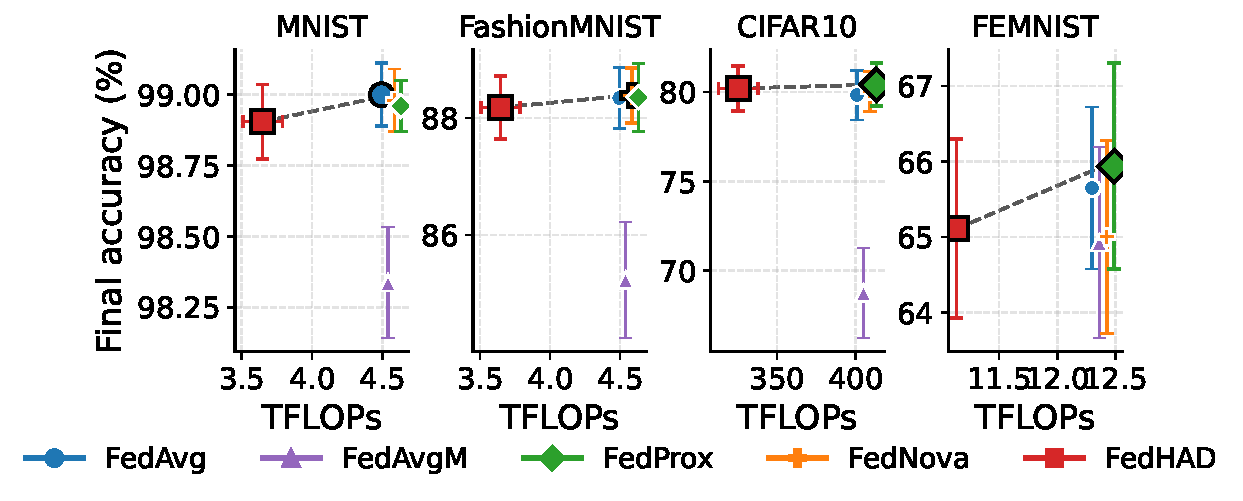
\includegraphics[width=\textwidth]{figures/figA_pareto_accuracy_compute.pdf}
  \caption{Final accuracy versus realised compute for each dataset. Larger
  markers with a black edge are on the Pareto front; dashed line connects the
  non-dominated points. Error bars are one standard deviation over 30 seeds.
  A method inside the front is dominated: another method reaches at least the
  same accuracy for no more compute. The four fixed-epoch baselines run at
  identical compute, so their markers are offset horizontally by a small fixed
  amount for legibility only; their true TFLOPs coincide and are listed exactly
  in Table~\ref{tab:acc-compute}.}
  \label{fig:pareto}
\end{figure*}

\begin{figure*}[t]
  \centering
  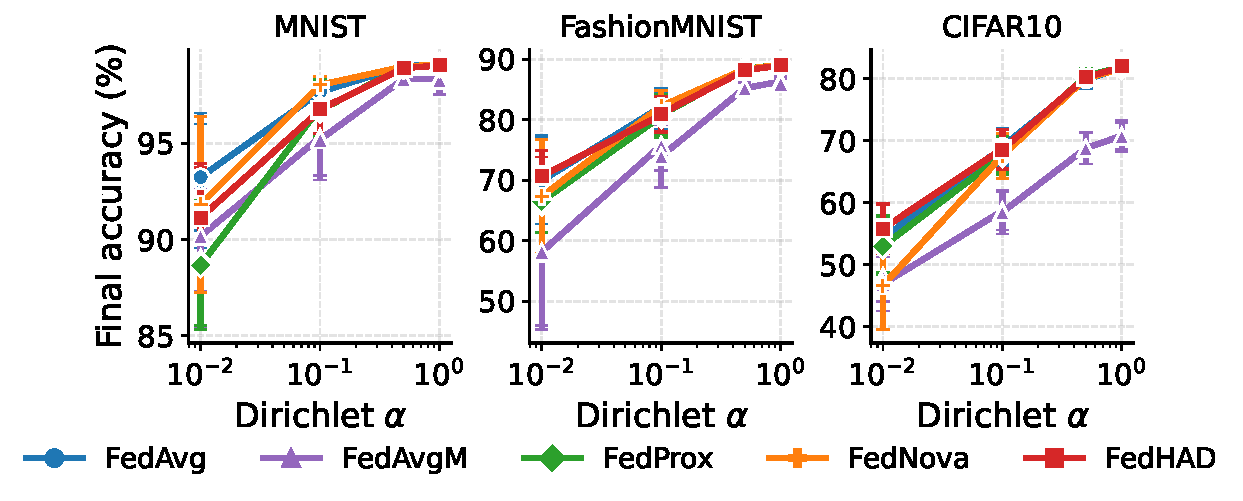
\includegraphics[width=\textwidth]{figures/figB_heterogeneity_severity.pdf}
  \caption{Final accuracy as Dirichlet $\alpha$ decreases. Combines the
  $\alpha=0.5$ and $\alpha=0.01$ base campaigns, executed on different
  platforms (Section~\ref{platforms}) and never compared pairwise.}
  \label{fig:heterogeneity}
\end{figure*}

\begin{figure*}[t]
  \centering
  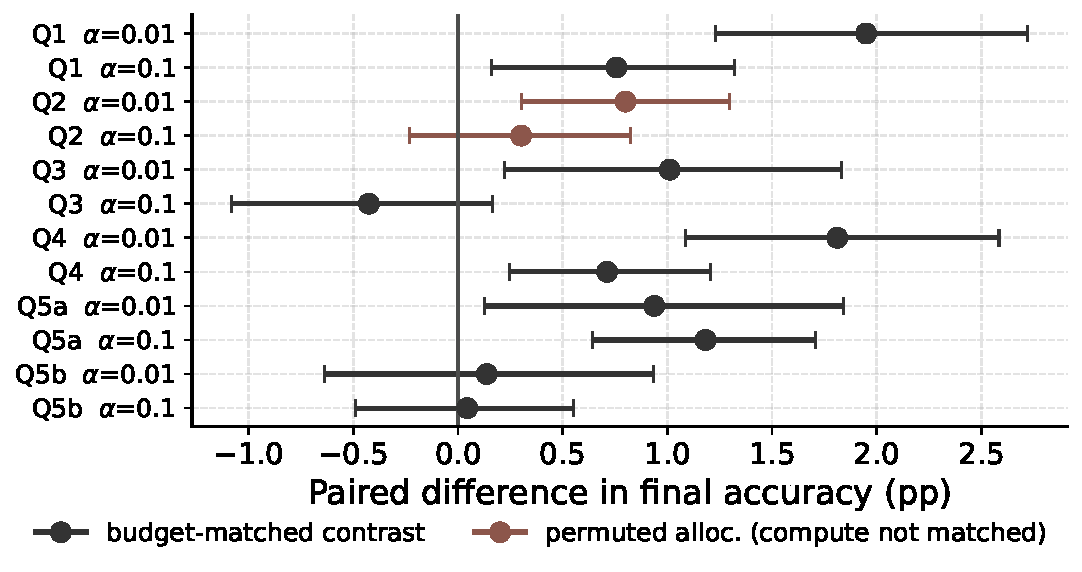
\includegraphics[width=\textwidth]{figures/figC_ablation_contrasts.pdf}
  \caption{Paired contrasts of the controlled ablation on CIFAR-10, 30 seeds,
  with 95\% bootstrap intervals over seeds. Blue contrasts have matched update budgets;
  the orange contrast uses \texttt{permuted\_allocation}, whose update budget is
  not matched and which is therefore complementary evidence only.}
  \label{fig:ablation}
\end{figure*}

